\documentclass[conference]{IEEEtran}

\usepackage{graphicx}
\usepackage{float}
\usepackage{afterpage}
\usepackage{hyperref}
\usepackage{listings}
\usepackage{import}
\usepackage{algorithm2e}
\usepackage{tabularx}
%\usepackage{syntax}
\usepackage[epsilon]{backnaur}
\usepackage{newfloat}

% bib
\bibliographystyle{IEEEtran}

% correct syntax bug
\AtBeginDocument{\catcode`\_=8 }

% correct bad hyphenation here
\hyphenation{op-tical net-works semi-conduc-tor}

% path to figures
\graphicspath{{figures/}}

% declare the floating environment {Grammar}
% this will also define \listofGrammars:
\DeclareFloatingEnvironment[
  % the file extension for the file used to create the list:
  fileext   = logr,% don't use log here!
  % the heading for the list:
  listname  = {List of Grammars},
  % the name used in captions:
  name      = Grammar,
  % the default floating parameters if the environment is used
  % without optional argument:
  placement = htp
]{Grammar}

\begin{document}

\title{Web Application Model Generation \\through Reverse Engineering and UI Pattern Inferring}

\author{
\IEEEauthorblockN{Clara Sacramento}
\IEEEauthorblockA{Department of Informatics Engineering,\\ Faculty of Engineering of the \\University of Porto \\Porto, Portugal \\ei09090@fe.up.pt}
\and
\IEEEauthorblockN{Ana C. R. Paiva}
\IEEEauthorblockA{INESC TEC, Department of Informatics Engineering, \\Faculty of Engineering of the \\University of Porto \\ Porto, Portugal \\apaiva@fe.up.pt}}


% use for special paper notices
%\IEEEspecialpapernotice{(Invited Paper)}

%ACP -------

% É preciso clarificar que não há contribuições na execução dos testes.
% tem que se fazer uma discussão dos resultados comparativos das duas diferentes abordagens
% dizer explicitamente qual é a research question %%%check
% ver o trabalho do Artemis (Mesbah)
% corrigir o abstract no que diz respeito aos modelos introduzirem bugs %%%check
% corrigir a informação do algoritmo 1
% Mudar o nome da subsecção para File Processing (LogProcessor) %%%check
% reformatar listing 1 %%%check
% explicar o que é o epsilon %%%check
% colocar refs de model/metamodel inference e de DSLs 


% verificar se é UITP ou UI patterns
%--------

% make the title area
\maketitle

\begin{abstract}
A great deal of effort in model-based testing is related to the creation of the model. In addition, the model itself, while a powerful tool of abstraction, can have conceptual errors, introduced by the tester. These problems can be reduced by generating those models automatically. This paper presents a dynamic reverse engineering approach that aims to extract part of the model of an existing Web application through the identification of User Interface (UI) patterns. This reverse engineering approach explores automatically any Web application, records information related to the interaction, analyzes the gathered information, tokenizes it, and infers the existing UI patterns via syntactical analyzing. After complemented with additional information and validated, the model extracted is the input for the Pattern-Based Graphical User Interface Testing (PBGT) approach for testing existing web application under analysis.
\end{abstract}
\begin{IEEEkeywords} Reverse Engineering, Web Application, UI Patterns, Web Scraping \end{IEEEkeywords}

\IEEEpeerreviewmaketitle

\section{Introduction}\label{sec:intro}

Web applications are getting more and more important, and can now handle tasks that before could only be performed by desktop applications \cite{garrett2005ajax}, like editing images or creating spreadsheet documents. However, despite their growing relevance, they still suffer from a lack of standards and conventions \cite{constantine2002usage}, unlike desktop and mobile applications. This means that the same task can be implemented in many different ways, which makes automated Web application testing difficult to accomplish and inhibits reuse of testing code. For instance, the authentication (\textit{login}) failure usually triggers the appearance of an error message, but some implementations simply erase the inserted data, with no error message visible.\\

% por exemplo o login válido pode implicar uma mudança de página ou uma mensagemd e erro ou simplesmente apagar a informação introduzida e continuar na mesma página
%%% check

Graphical User Interfaces (GUI) of all kinds are populated with recurring behaviors that vary slightly, an example being authentication (\textit{login/password}) and content search. These behaviors (patterns) are called User Interface (UI) patterns \cite{van2001patterns} and are recurring solutions that solve common design problems. Due to their widespread use, UI patterns allow users a sense of familiarity and comfort when using applications. \\

However, while UI patterns are familiar to users, their implementation may vary significantly.  Despite this, it is possible to define generic and reusable test strategies (User Interface Test Patterns - UITP) to test those patterns. This requires a configuration process, in order to adapt the tests to different applications \cite{morgado2012gui}. \\

That is the main idea behind the PBGT (\textit{Pattern-based GUI Testing}) project, in which this research work is included. In the PBGT approach, the user builds a test model of the Web application with instantiations of UI Test Patterns, and later uses that model to test the Web application. The model can be built manually by the user, but this is a morose process and not recommended, since it may introduce conceptual errors. Half the bugs found through model-based testing are conceptual errors in the model itself and not bugs in the system to test \cite{dalal1999model}.\\

The goal of the work described in this paper is to continue the work done in \cite{nabuco2013inferring} on the reverse engineering process (PARADIGM-RE). More specifically, this research work aims to automatize the model construction: independently/automatically explore a Web application, infer the existing UI patterns in its pages, and finally produce a model with the UI Test Patterns that define the strategies to test the UI Patterns present in the web application. This speeds up model construction, and hopefully introduces less errors into the model.\\

The rest of the paper is structured as follows. Section \ref{sec:pbgt} presents an overview of the PBGT project, setting the context for this work.  Section \ref{sec:re} describes the developed approach, its components and  their interrelations, and the results it produces. Section \ref{sec:eval} provides a practical example of the proposed system. Section \ref{sec:sota} addresses the related work, as well as the available tools to perform the needed tasks. Section \ref{sec:conc} presents the conclusions, some of the problems encountered and a perspective on future work. \\

\section{PBGT Overview}\label{sec:pbgt}

As mentioned before, the focus of this paper is the reverse engineering component of a research project named PBGT (\textit{Pattern-based GUI Testing}) \cite{moreira2013pattern}. The goal of this project is to develop a model-based GUI testing approach and supporting tool, that can be used in industrial contexts.\\

\subsection{Architecture}
The PBGT supporting toolshas main five components: 
\begin{enumerate}
\item \textbf{PARADIGM}, a DSL (\textit{Domain Specific Language}) to define GUI testing models based on UI Test Patterns \cite{enase14}; 
\item \textbf{PARADIGM-RE}, a Web application reverse engineering tool whose purpose is to extract UI patterns from Web pages without access to their source code, and use that information to generate a test model written in PARADIGM; 
\item \textbf{PARADIGM-ME}, a modeling and testing environment, built to support the creation of test models \cite{conf_icst_MonteiroP13}; 
\item  \textbf{PARADIGM-TG}, an automatic test case generation tool that generates test cases from test models defined in PARADIGM according to coverage criteria selected by the tester; 
\item and finally, a test case execution tool, named \textbf{PARADIGM-TE}, which executes test cases, analyzes their coverage with a coverage analysis tool named \textbf{PARADIGM-COV}\cite{vilela2014cov}, and returns detailed execution reports. 
\end{enumerate}

The architecture and workflow of the project is shown in Fig. \ref{fig:pbgt}.
\begin{figure}[!htb]
\centering
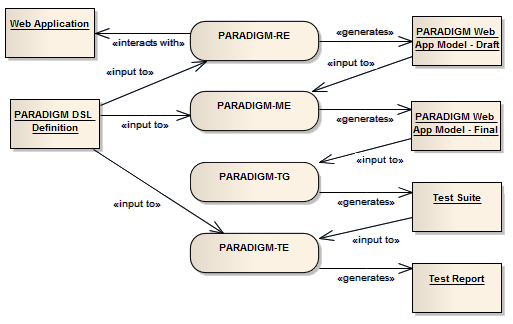
\includegraphics[width=0.5\textwidth]{pbgt}
\caption{An overview of the PBGT project.}
\label{fig:pbgt}
\end{figure}

\subsection{PARADIGM DSL}\label{sec:dsl}
%falar doc conetores e, do init e do end, e falar também dos elementos estruturais: Form e Group

PARADIGM is a DSL to be used in the domain of PBGT. The goal of the language is to gather applicable domain abstractions (e.g., UI test patterns), allow specifying relations between them and also provide a way to structure the models in different levels of abstraction to cope with complexity. PARADIGM's meta-model is illustrated in Figure \ref{fig:dsl}.\\
\begin{figure}[!htb]
\centering
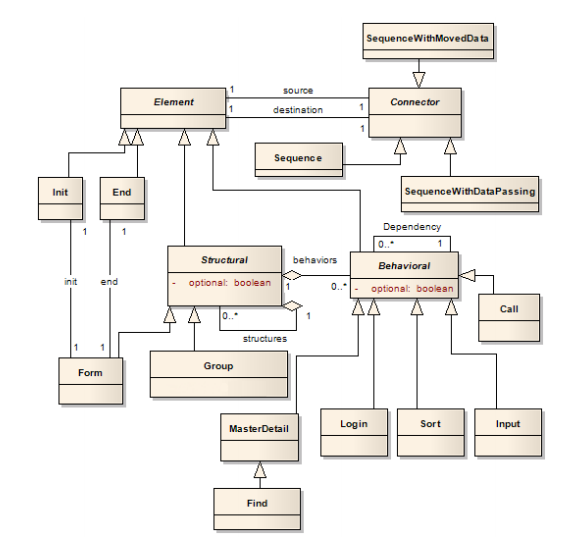
\includegraphics[width=0.52\textwidth]{dsl}
\caption{PARADIGM DSL Meta-model.}
\label{fig:dsl}
\end{figure}

The PARADIGM language is comprised by elements and connectors \cite{moreira2013pattern}. There are four types of elements: \textit{Init} (to mark the beginning of a model), \textit{End} (to mark the termination of a model), \textit{Structural} (to structure the models in different levels of abstraction), and \textit{Behavioral} (UI Test Patterns describing the testing goals).\\

As models become larger, coping with their growing complexity forces the use of structuring techniques such as different hierarchical levels that allow use one entire model \textbf{A} inside another model \textbf{B} abstracting the details of \textbf{A} when within \textbf{B}. Structuring techniques are common in programming languages like C and Java, with constructs such as modules and classes. \textit{Form} is a structural element that may be used for that purpose. A \textit{Form} is a model (or sub-model) with an \textit{Init} and an \textit{End} elements. \textit{Group} is also a structural element but it does not have \textit{Init} and \textit{End} and, moreover, all elements inside the \textit{Group} are executed in an arbitrary order.\\

\begin{figure}[!htb]
\centering
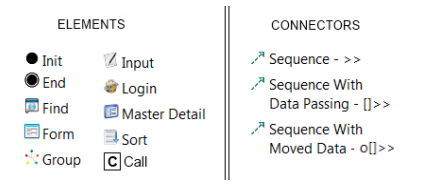
\includegraphics[width=0.5\textwidth]{dsl1}
\caption{PARADIGM syntax.}
\label{fig:dsl1}
\end{figure}

PARADIGM elements and connectors are described by: (i) an icon/figure to represent the element graphically and (ii) a short label to name the element. The overall syntax of the DSL is illustrated in Figure \ref{fig:dsl1}. Additionally, elements within a model have a number to identify them, and optional elements have a ``op" label next to its icon/figure.\\

This language has three connectors: \textit{Sequence}, \textit{SequenceWithDataPassing}, and \textit{SequenceWithMovedData}. \textit{Sequence} indicates that the testing strategy related to the target element cannot start until the testing strategy of the source element has completed. \textit{SequenceWithDataPassing} has the same meaning as \textit{Sequence}, and additionally indicates that the target element receives data from the source element. \textit{SequenceWithMovedData} has a similar meaning to \textit{SequenceWithDataPassing}, but the source element moves data to the target instead of transferring a copy. In addition, there is another kind of relation among elements -- \textit{Dependency} -- indicating that the target element depends on the properties of a set of source elements, for instance, when it is the result of a calculation. \\

A UI Test Pattern defines a test strategy which is formally defined by a set of test goals (for later configuration)\cite{moreira2013pattern} with the form:

\begin{equation}< Goal; V; A; C; P >\end{equation}\label{eq:ui_}

\textit{Goal} is the \textit{ID} of the test. \textit{V} is a set of pairs { [\textit{variable}, \textit{inputData}] } relating test input data with the variables involved in the test. \textit{A} is the sequence of actions to perform during test case execution. \textit{C} is the set of possible checks to perform during test case execution, for example, “check if it remains in the same page”. \textit{P} is a Boolean expression (precondition) defining the set of states in which it is possible to execute the test. The language also defines language constraints to guarantee the building of well-formed models, such as ``\textit{A Connector cannot connect an element to itself}'' and ``\textit{A Connector cannot have Init as destination, or End as source}'', to cite a few examples.\\

The UI Patterns defined in the PARADIGM language are:
\begin{itemize}
\item \textbf{Login}: This pattern is commonly found in Web applications, especially in the ones that restrict access to functionalities or data. Usually consists of two input fields (a normal input box for email or username, and a cyphered text for the password) and a submit button, with optionally a ``remember me'' checkbox. The authentication process has two possible outcomes: valid and invalid. Upen authintication failure a message may be shown. 
\item \textbf{Find}: This pattern consists of one or more input fields, where the user inserts keywords to search, and a submit button to start the search. The search may be submitted via a submit button, or dynamically upon text insertion. When the search is successful, the website shows a list of results; upon failure, an error message may be shown.
\item \textbf{Sort}: This pattern sorts a list of data by a common attribute (e.g., price, name, relevance, etc.) according to a defined criteria (ascending or descending, alphabetically, etc.).
\item \textbf{Master Detail}: This pattern is present in a webpage when selecting an element from a set (called \textit{master}) results in filtering/updating another related set (called \textit{detail}) accordingly. For example, clicking on a checkbox associated to a brand may include (or exclude) products of that brand in a product search result list. Generally the only elements changed are the elements belonging to the \textit{detail} set.
\item \textbf{Call}: This pattern is any kind of element where a click triggers some procedure that may result in a change of page.
\end{itemize}

\subsection{Produced Models}

The models produced by the reverse engineering tool PARADIGM-RE consist of a XML file in the format required by the PARADIGM-ME which contains information about the UI Test Patterns needed to test the UI Patterns found: their name, the input values for their variables, i.e., the values used during the exploration process, and blank pre-conditions and checks for the tester to fill in. The UI Test Patterns within the model are connected in a linear path according to the exploration order. The testing configuration information needs to be complemented and validated by the tester afterwards in order to generate test cases and execute them over the web application under analysis.

\section{Reverse Engineering Approach}\label{sec:re}

\subsection{Previous Tool}\label{sec:prev}

The  approach described in this paper aims to improve on the previous work \cite{nabuco2013inferring} done on the PARADIGM-RE tool. In particular it aims to be fully automatic. The previous tool required the intervention of the user to interact with the web application under analysis in order to save the interaction traces and proceed from there. It extracted information from an user's interaction with the Web application under analysis, analysed the information, produced some metrics (such as the total ratio of the LOC (\textit{lines of code}), length of all visited pages and the ratio of two subsequent pages), and finally used those metrics and the user interaction's information to infer UI patterns via a set of heuristic rules. \\

The information saved from a user interaction was the source code and URLs of the visited pages, and the interaction's execution trace. An execution trace is the sequence of user actions executed during the interaction with a software system, such as clicks, text inputs and also some information of the system state (e.g., the information that is being displayed). An example of an execution trace file used by the tool can be seen in Table \ref{tab:exec}.\\

\begin{table}[!htb]
\resizebox{0.5\textwidth}{!}{
  \begin{tabular}{| c | c | c |}
     \hline
     \textbf{Action} & \textbf{Target} & \textbf{Value} \\ \hline
     type&id=input\_username &``user1" \\ \hline
     type&id=input\_password &``123pass" \\ \hline
     clickAndWait & css=input[type=``submit"]&EMPTY \\
     \hline
     type&id=searchInput&``coffee" \\ \hline
	 clickAndWait & id=mw-searchButton&EMPTY\\
     \hline
     select&id=sort&label=Price:Low to High \\
     \hline
     %%%%%
     click&id=collapseButton1&EMPTY\\\hline
     click&link=Next&EMPTY\\\hline
     typeAndWait&id=freeSearch&ministry\\\hline
     type&id=authcode&T75Y5\\\hline
     type&name=firstName&james\\\hline
	 type&name=lastName&bond\\\hline
     click&//ul[@id='ref1']/li[5]/a/span&EMPTY\\\hline
  	 \end{tabular}
}
\caption{Example of an execution trace file.}
\label{tab:exec}
\end{table}

The previous reverse engineeing approach identified the \textit{Find}, \textit{Login}, \textit{Sort}, \textit{Input} and \textit{MasterDetail} patterns, and produced a high number of false positives \cite{nabuco2013inferring}. Aditionally, and as already mentioned, the exploration process was done by saving the user interaction with the Web application under test, requiring human interaction to identify patterns. The results were dependent on the execution traces followed by the tester. \\

\subsection{Current Tool}

The work described in this paper has the same primary aim as the previous tool (to identify UI patterns in the Application Under Test (AUT)), but has other goals. The first is to remove the need for user interaction with the AUT to identify patterns, by providing a reverse engineering process to explore automatically the web application under analysis. The second is to refine and improve the pattern inferring process, and lower or eliminate completely the percentage of false positives. The third is to identify more patterns than the previous tool.\\

The architecture of the tool is seen in Figure \ref{fig:retool}.
\begin{figure}[!htb]
\centering
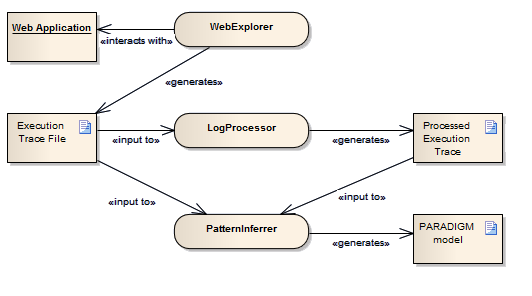
\includegraphics[width=0.5\textwidth]{retool}
\caption{The architecture of the approach.}
\label{fig:retool}
\end{figure}

The approach can be divided into three parts: \textbf{WebsiteExplorer}, \textbf{LogProcessor}, and \textbf{PatternInferrer}.

\textbf{WebsiteExplorer} loads user configurations (more details on Section \ref{sec:conf}), interacts automatically with the AUT and produces an execution trace file with the actions taken (see Table \ref{tab:exec} for an example). \textbf{LogProcessor} is a text parser. It analyzes the previous file, parses each line, searches for important keywords and uses them to identify the action contained in the line, and produces an updated execution trace file (see Table \ref{tab:exec1} for an example). Finally, \textbf{PatternInferrer} analyzes the updated execution file, identifies the existent patterns, their location in the website and any existing parameters, and produces an XML file with the results. The patterns identifiable by this tool are all of those defined in the PARADIGM language, plus the \textit{Menu} UI pattern. \\

\subsection{AUT Exploration (WebsiteExplorer)}\label{sec:inter}
The interaction process is described in a simplified manner in Algorithm \ref{alg:seeker}.

\begin{algorithm}
  %\SetLine
  \KwData{number\_of\_actions, number\_of\_iterations, website\_base\_url, configuration\_file}
  \KwResult{execution\_trace\_file}
  
  current\_action := 0; redirections := 0\;
  configuration := parseConfigurationFile()\;
  
  \While{current\_action $<$ configuration.number\_of\_actions}{
    \If{configurations.isSearchingForMenu()}
      {
        menuElements.add(getMenuElementsInPage())\;
      }
    \If{configuration.isSearchingForMasterDetail()}
    {
      masterElements.add(getMasterElementsInPage())\;
      detailElements.add(getDetailElementsInPage())\;
    }
  
  	list := extractValidNonVisitedElements\;
    next\_element := chooseNextElement(list)\;
  \eIf{next\_element == null}
  {%then
  	redirections++\;
    \eIf{redirection $<$ configuration.number\_of\_iterations}
    	{%then
        	go\_to\_base\_URL\;
            write\_to\_execution\_trace\_file\;
        }
        {%else
        	end\_program\;
        }
  }
  {%else
  	visit(element)\;
    visitedElements.add(element)\;
    write\_to\_execution\_trace\_file\;
    current\_action++;
    wait(configuration.politenessDelay)\;
  }
}

\caption{Pseudo-code algorithm to explore a page.}\label{alg:seeker}
\end{algorithm}

Currently the elements explored are \textit{$<$select$>$} elements, \textit{$<$input$>$} elements, and \textit{$<$a$>$} (link) elements. The way each element is visited is different: link elements are clicked; input elements get text (either a keyword or a number, depending on the type of input) and the containing form is submitted; and in the case of dropdown menus, a random option is selected and the surrounding form is submitted. The exception to the \textit{input} rule is when the element is identified as a \textit{login} element, in which case all the sibling elements (elements inside the form where the selected element is located) get text and only then the form is submitted.\\

Information about these elements is extracted via XPath\footnote{XPath: \url{www.w3schools.com/XPath/}}. Before interacting with an element, the algorithm makes the following checks: if the element has not been visited in the current page, and if the element contains any unwelcome keywords that if explored may drive the explorer into unwanted paths. These keywords may be general to all elements (anything that edits information or contains the words 'buy'/'sell', for example, that would lead to purchase products) or element-specific (input elements cannot contain the attribute '\textit{disabled}' or'\textit{readonly}', if they are to be interacted with). All elements have the same probability of being chosen from a list of elements.\\

The execution trace file produced is a CSV (\textit{Comma-separated values}) file with three columns: \textbf{action}, the type of action executed (\textit{click, type}, or \textit{select} when selecting an option in a dropdown menu -- it may also contain the suffix \textit{AndWait}, which indicates a page change); \textbf{target}, the identifier of the visited element; and \textbf{value}, which has the parameter for the action and may be empty (for example, in the case of \textit{type} actions, it is the inserted text).\\

The exceptions are the Menu and MasterDetail patterns. Since the explorer cannot be relied on to explore every element belonging to these patterns in each page, elements belonging to these patterns are found through analysing the current page source and extracting all elements that obey a set of rules. For the Menu pattern, the anchor links that are in \textit{$<$nav$>$}, \textit{$<$header$>$} or \textit{$<$footer$>$} tags are automatically included as part of the Menu pattern. Besides this, Menu elements and Master Detail are identified by a set of identifiers passed via the configuration file, and they are identified as its respective pattern if they respect the condition \texttt{(//*[contains(@class,identifier)] OR //*[contains(@id,identifier)] OR //*[contains(@name,identifier)])}.\\

The results of the HTML analysis are passed directly to the \textbf{PatternInferrer} to be written in the final output file (see Section \ref{sec:inf}).\\

\subsection{Configuration}\label{sec:conf}
To improve results, almost all components used in the website interaction and pattern identifying processes can be loaded to the application via a XML configuration file, the only exception being the PatternInferrer grammar. This is done to allow the maximum flexibility to the tester to adjust the tool to the web application to test.\\

The components and values that can be loaded via configuration file are: 
\begin{itemize}
\item[] \textbf{actions}: number of actions the crawler will execute before stopping;
\item[] \textbf{redirections}: number of redirects to the home page the crawler will do before stopping; 
\item[] \textbf{politenessDelay}: time to wait (in milliseconds) after each action;
\item[] \textbf{typedKeywords}: list of words to insert in text input elements;
\item[] \textbf{searchKeywords}: regex with keywords that identify search elements;
\item[] \textbf{sortKeywords}: regex with keywords that identify sort elements;
\item[] \textbf{loginKeywords}: regex with keywords that identify login elements;
\item[] \textbf{generalWordsToExclude}: regex with keywords that mark elements that should not be accessed;
\item[] \textbf{menuIdentifiers}: list of ids/classes/names that identify menu elements;
\item[] \textbf{masterIdentifiers}: list of ids/classes/names that identify master elements;
\item[] \textbf{detailIdentifiers}: list of ids/classes/names that identify detail elements;
\item[] \textbf{historyFilepath}: specify absolute filepath for history file;
\item[] \textbf{processedHistoryFilepath}: specify absolute filepath for processed history file;
\item[] \textbf{patternsFilepath}: specify absolute filepath for PARADIGM model file;
\item[] \textbf{patternsToFind}: list of patterns that the explorer can search for - if "all" occurs, there will be no restriction;
\item[] \textbf{loginConfiguration}: credentials for a correct login in the web app;		
\item[] \textbf{tokenizerPatterns}: patterns for LogProcessor;
\item[] \textbf{includeChildrenNodesOnInteraction}: boolean; on interaction with an input or select element, if children elements should be included  in the history file, but not interacted with;
\end{itemize}

\subsection{Action File Processing (LogProcessor)}\label{sec:fp}

This component is a lexical analyzer, whose role is to examine the execution trace file line by line and identify the type of each action written therein. It has a data structure (which serves as its lexical grammar) containing the rules it is going to search for, and each has the following attributes: \textbf{pattern\_name}, the identifier for the rule; \textbf{identifying\_regex}, and a regex (Regular Expression\footnote{Regex: \url{http://www.regular-expressions.info/}}) that identifies an action of that type. \\

For every line, not all rules are tested; if a rule matches the line, first a camel-case token (composed by the sum of the action type and the rule's name) is produced, added to the processed trace file, and then the program moves on to the next line. If no rules match, only the action is written on the file. An example of file processing may be seen in Table \ref{tab:exec}.\\

\begin{table}[!htb]
\resizebox{0.5\textwidth}{!}{
  \begin{tabular}{| c | c | c || c |}
     \hline
     \textbf{Action} & \textbf{Target} & \textbf{Value} & \textbf{Processing Return} \\ \hline
     type&id=input\_username &user1&typeUsername \\ \hline
     type&id=input\_password &123pass&typePassword \\ \hline
     clickAndWait & css=input&EMPTY&clickFormSubmit \\
      & [type=``submit"] & & PageChange\\
     \hline
     type&id=searchInput&coffee&typeSearch \\ \hline
	 clickAndWait & id=mw-searchButton&EMPTY&clickSearch\\
      & & & PageChange \\ \hline
     select&id=sort&label=Price: &selectSort \\
      & & Low to High& \\
     \hline
     %%%%%%
     click&id=collapseButton1&EMPTY&clickCollapse\\ \hline
     click&link=Next&EMPTY&clickNextLink \\ \hline
     typeAndWait&id=freeSearch&ministry&typeSearch \\
      & & & PageChange \\ \hline
     type&id=authcode&T75Y5&typeAuth\\\hline
     type&name=firstName&james&typeFirstName\\\hline
	 type&name=lastName&bond&typeLastName\\\hline
     click&//ul[@id='ref\_679781011']/li[5]/a/span&EMPTY&click\\\hline
  	 \end{tabular}
} 
\caption{Example of an execution trace file, and of processed lines.}
\label{tab:exec1}
\end{table}

The identifiable tokens by default are: \textit{login, username, email, password, verifyPassword, submit, captcha, auth, search, sort, link, option, checkbox, radio, homeLink, imageLink, nextLink, prevLink, firstLink, lastLink, languageLink, buttonLink, searchResultLink, link, collapse, firstNameInput, lastNameInput, numberInput, input, button}, and \textit{clear}. However, the identifiable patterns can also be overridden and added to via a configuration file (see Section \ref{sec:conf}).\\

The tokens produced by the LogProcessor affect the pattern inferring done by PatternInferrer. For example, the patterns involved in the inferring of the Login pattern are \textit{username, email, login} (these identify username and email inputs, and login inputs or actions, depending on which action the token is appended to), \textit{password} (which identifies a password input),  and \textit{submit}, which are used to indicate the closing of a classical form submit action (when \textit{matchSubmit(line)} is true), and thus, the end of a standard pattern. Some patterns are identified to distinguish between proper patterns and other types of action non relevant to the inferring process, such as \textit{verifyPassword}, which can be used to distinguish between a Login form and a Register form, and \textit{searchResultLink}, which prevents search result links from being marked as part of a Find pattern. Some exist simply to give better context to the action, like \textit{nextLink} or \textit{lastName}.\\

\subsection{UI Pattern Inferring (PatternInferrer)}\label{sec:inf}

This component is a syntactical analyzer, that takes as input the extended execution trace file returned by the \textit{LogProcessor}, runs it against a predefined grammar, and returns the patterns found. The processing rules are formalized in Table \ref{tab:grammar}.

\begin{table}[!htb]
%\begin{bnf*}
\begin{tabular}{rcl}
  $\bnfpn{pattern}$ & $\bnfpo$ & $\bnfpn{login}$ $\bnfor$ $\bnfpn{find}$ $\bnfor$ $\bnfpn{sort}$ $\bnfor$ $\bnfpn{input}$ $\bnfor$ $\bnfpn{call}$ \\
  
  $\bnfpn{find}$  & $\bnfpo$ &  $\bnfpn{match-find}$ $\bnfsp$ $\bnfpn{opt-submit}$ \\
  
  $\bnfpn{sort}$ & $\bnfpo$ &  $\bnfpn{match-sort}$ $\bnfsp$ $\bnfpn{opt-submit}$ \\
  
  $\bnfpn{input}$ & $\bnfpo$ &  $\bnfpn{match-input}$ $\bnfsp$ $\bnfpn{opt-submit}$ \\
  
  $\bnfpn{call}$ & $\bnfpo$ &  $\bnfpn{match-link}$ $\bnfsp$ $\texttt{PageChange}$ \\
  
  $\bnfpn{login}$ & $\bnfpo$ &  $\bnfpn{opt-login-rec}$ $\bnfsp$ $\bnfpn{match-user-pass}$\\
  & & $\bnfsp$ $\bnfpn{match-submit}$ \\
  
  $\bnfpn{match-user-pass}$ & $\bnfpo$ &  $\bnfpn{match-user}$ $\bnfsp$ $\bnfpn{match-pass}$ \\
  & & $\bnfor$ $\bnfpn{match-pass}$ $\bnfsp$ $\bnfpn{match-user}$ \\
  
  $\bnfpn{opt-submit}$ & $\bnfpo$ &  $\bnfpn{match-submit}$ $\bnfor$ $\bnfes$ \\
  
  $\bnfpn{match-submit}$ & $\bnfpo$ &  $\texttt{clickFormSubmit}$ $\bnfor$ $\texttt{clickButton}$ \\
  
  $\bnfpn{match-find}$ & $\bnfpo$ &  $\bnfpn{opt-find-rec}$ $\bnfsp$ $\bnfpn{search-item}$ $\bnfsp$ $\bnfpn{opt-find-rec}$ \\
  
  $\bnfpn{match-sort}$ & $\bnfpo$ &  $\texttt{clickSort}$ $\bnfor$ $\texttt{selectSort}$ \\
  
  $\bnfpn{match-input}$ & $\bnfpo$ &  $\texttt{clickInput}$ $\bnfor$ $\texttt{typeInput}$ \\
  & & $\bnfor$ $\texttt{typeNumberInput}$ \\ 
  & & $\bnfor$ $\texttt{typeFirstNameInput}$ \\
  & & $\bnfor$ $\texttt{typeLastNameInput}$ \\
  
  $\bnfpn{match-user}$ & $\bnfpo$ &  $\bnfpn{opt-login-rec}$ $\bnfsp$ $\bnfpn{user}$ $\bnfsp$ $\bnfpn{opt-login-rec}$ \\
  
  $\bnfpn{match-pass}$ & $\bnfpo$ &  $\bnfpn{opt-login-rec}$ $\bnfsp$ $\bnfpn{pass}$ $\bnfsp$ $\bnfpn{opt-login-rec}$ \\
  
  $\bnfpn{user}$ & $\bnfpo$ &  $\texttt{typeUsername}$ \\
  & & $\bnfor$ $\texttt{typeEmail}$ $\bnfor$ $\texttt{typeLogin}$ \\
  
  $\bnfpn{pass}$ & $\bnfpo$ &  $\texttt{typePassword}$ \\
  
  $\bnfpn{match-opt-login}$ & $\bnfpo$ &  $\texttt{clickLogin}$ $\bnfsp$ $\texttt{PageChange}$ \\
  & & $\bnfor$ $\texttt{typeAuth}$ $\bnfor$ $\texttt{typeCaptcha}$ \\
  & & $\bnfor$ $\texttt{clickOption}$ $\bnfor$ $\texttt{clickRadio}$ \\
  
  $\bnfpn{match-link}$ & $\bnfpo$ &  $\texttt{clickLink}$ \\
   & & $\bnfor$ $\texttt{clickHomeLink}$ \\
   & & $\bnfor$ $\texttt{clickImageLink}$ \\
   & & $\bnfor$ $\texttt{clickNextLink}$ \\
   & & $\bnfor$ $\texttt{clickPrevLink}$ \\
   & & $\bnfor$ $\texttt{clickFirstLink}$ \\
   & & $\bnfor$ $\texttt{clickLastLink}$ \\
   & & $\bnfor$ $\texttt{clickLanguageLink}$ \\
   & & $\bnfor$ $\texttt{clickButtonLink}$ \\
   & & $\bnfor$ $\texttt{clickSearchResultLink}$ \\
  
  $\bnfpn{opt-find-rec}$ & $\bnfpo$ &  $\bnfpn{opt-find-rec}$ $\bnfor$ $\bnfpn{opt-search}$ \\
  & & $\bnfor$ $\bnfpn{search-item}$ $\bnfor$ $\bnfes$ \\
  
  $\bnfpn{opt-search}$ & $\bnfpo$ &  $\texttt{clickSearch}$ \\
  
  $\bnfpn{search-item}$ & $\bnfpo$ &  $\texttt{typeSearch}$ $\bnfor$ $\texttt{selectSearch}$ \\
  
  $\bnfpn{opt-login-rec}$ & $\bnfpo$ &  $\bnfpn{opt-login-rec}$ $\bnfor$ $\bnfpn{match-opt-login}$ $\bnfor$ $\bnfes$ \\
  & & \\
  \end{tabular}
%\end{bnf*}
\caption{Default grammar used by LogProcessor to tokenize the execution trace file ($\epsilon$ indicates an empty string).}
\label{tab:grammar}
\end{table}

If during the process the tool detects the same UI Pattern instance several times, the tool is capable of ignoring the repetitions. Its reasoning is explained in Figure \ref{fig:inferrer}.\\

\begin{figure}[!htb]
\centering
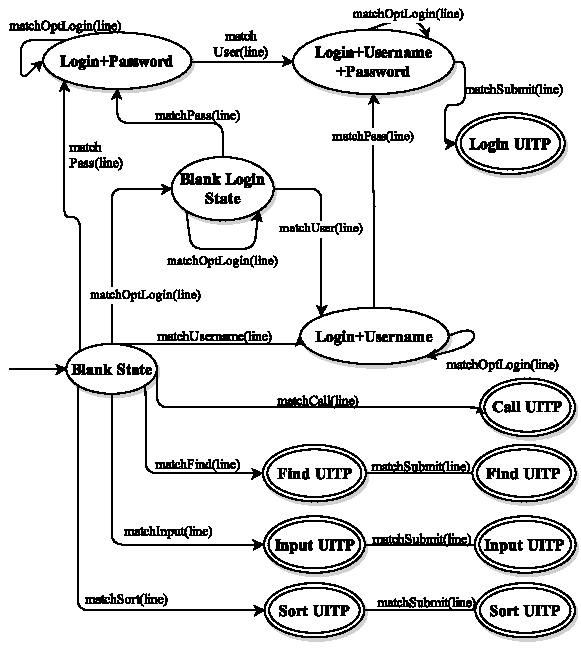
\includegraphics[width=0.5\textwidth]{Global_State_Machine.pdf}
\caption{The inferrer's reasoning algorithm, expressed in a finite state machine.}
\label{fig:inferrer}
\end{figure}

For simplicity's sake, only the valid paths are shown in the figure (Fig. \ref{fig:inferrer}). All patterns except \textit{Login} can be valid even in the absence of a form submit action; this is done to account for dynamic submission via Javascript. In the case of the Login pattern, there can only be one password and one username or email record; this is done to distinguish login forms from register forms and password/email change forms.\\

The previous figure (Fig. \ref{fig:inferrer}) does not account for the \textit{Menu} and \textit{Master Detail} patterns; as mentioned before, these patterns are identified through HTML analysis and passed directly from the \textit{WebsiteExplorer} to the \textit{PatternInferrer} to write. This grammar only deals with the patterns identifiable through the execution trace file.\\

After the file is processed, an XMI file is produced containing all the pattern occurrences found, and the values assigned to each variable, as per Formula 1.%\ref{eq:ui_}. 
As mentioned before, the checks to perform within each test strategy and any preconditions must be specified by the tester later on in the PARADIGM-ME tool.\\

An example of a execution trace file extract from which a Login pattern can be inferred can be seen in Table \ref{tab:fullpattern}.

\begin{table}[!htb]
\resizebox{0.5\textwidth}{!}{
\begin{tabular}{|c|c|c|c|}
\hline
\textbf{Action} & \textbf{Target} & \textbf{Value} & \textbf{Processing Return} \\ \hline
 & //a[@class=active &	 &  \\
clickAndWait & and @href=\ldots & EMPTY & clickLogin pageChange\\
&  and contains(text(),'Login')] & &  \\\hline
 & //input[@id=email & &  \\
type&  and @name=email & login@en.pt  & typeEmail\\
&  and @type=text] & & \\\hline
 & //input[@id=password  & &  \\
type& and @type=password & pass & typePassword\\
& and @name=password] & & \\\hline
 & //input[@id=save\_login &  &   \\
click& and @name=save\_login & EMPTY & clickLogin\\
&  and @type=checkbox] & & \\\hline
 & //input[@class=btn\_small grey &  &  \\
clickAndWait& and @name=commit & EMPTY & clickSubmit pageChange \\
&  and @type=submit] & & \\\hline
\end{tabular}
}
\caption{Execution trace example from which a Login pattern can be inferred.}
\label{tab:fullpattern}
\end{table}

\section{Evaluation}\label{sec:eval}

In order to evaluate the developed reverse engineering approach, some experiments were performed. They aimed to answer the following research questions.

\subsection{Research Questions}
\begin{itemize}
  \item[R1)] Is it possible to infer automatically UI Patterns from a Web application?\\
  \item[R2)] Is it possible to improve the results provided by the previous RE tool?\\
\end{itemize}

\subsection{Evaluation Results}

The RE tool was initially experimented iteratively over a set of Web applications, with the goal of refining and fine-tuning the inferring grammars used to find UI Patterns.

Afterwards, the RE tool was used to detect UI Patterns in several public known and widely used Web applications, in an evaluation set. This time, the purpose was to evaluate the RE tool, i.e., determine which UI pattern occurrences the tool was able to detect in each application execution trace (ET) and compare them to the patterns that really exist in such trace.

Five applications were chosen from the most popular Websites\footnote{according to: \url{en.wikipedia.org/wiki/List_of_most_popular_websites‎}}: Amazon, Wikipedia, Ebay, Youtube, Facebook and Yahoo.

The results of the experiments are presented in table \ref{tab:eval_curr}. It shows the number of instances of each UI pattern that exist in the execution traces, the ones that the tools correctly found and the ones that the tools mistakenly found (false positives). 

\begin{table}[!htb]
\resizebox{0.5\textwidth}{!}{
  \begin{tabular}{| c | c | c | c | c |}
    \hline \multicolumn{5}{|c|}{\textbf{Current Tool}} \\ \hline
     \textbf{Pattern} & \textbf{Present} & \textbf{True} & \textbf{False} & \textbf{False} \\
       & \textbf{in ET} & \textbf{Positive} & \textbf{Negative} & \textbf{Positive} \\ \hline
     Login & 4 & 4 & 0 & 0 \\
     Find & 15 & 13 & 2 & 0 \\
     Sort & 1 & 1 & 0 & 0 \\
     Input & 29 & 28 & 1 & 0 \\
     Call & 249 & 235 & 14 & 0 \\ 
     Menu & 212 & 216 & 0 & 4 \\
     MasterDetail & 58 & 46 & 12 & 0 \\ \hline
     \textbf{Total} & \textbf{568 (100\%)} & \textbf{543 (95.59\%)} & \textbf{29 (5.1\%)} & \textbf{4 (0.7\%)} \\ \hline
  \end{tabular}
}
\caption{Evaluation set results from the current tool.}
\label{tab:eval_curr}
\end{table}

As we can see in Table \ref{tab:eval_curr}, the reverse engineering tool found few false positives, most related to the Menu UI Pattern. In addition it is worth to mention that the tool found 95.59\% of the  patterns present in the automatically explored execution traces.

However, the case study does not mention how many patterns were present in the web applications that were not visited, which we have not verified. Only one path produced by the application was considered for each Web application, and all the paths were run using the standard configuration, excluding any login credentials included.

A simplified version of one of the generated models can be seen in Figure \ref{fig:pbgt-me}.

\begin{figure}[!htb]
\centering
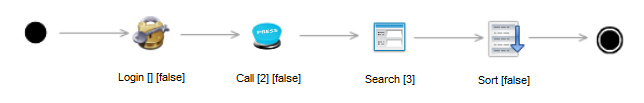
\includegraphics[width=0.5\textwidth]{pbgt-me.png}
\caption{A simplified example of a generated model.}
\label{fig:pbgt-me}
\end{figure}

\section{Related Work}\label{sec:sota}

Reverse engineering is ``the process of analyzing the subject system to identify the system components and interrelationships and to create representations of the system in another form or at a higher level of abstraction'' \cite{chikofsky1990reverse}. There are four methods of applying reverse engineering to a system: the dynamic method, in which the data is retrieved from the system at run time without access to the source code, the static method, which obtains the data from the system source code \cite{systa1999dynamic}, the hybrid method, which combines the two previous methods, and the historical method, which extracts information about the evolution of the system
from version control systems, like SVN\footnote{SVN: svn.apache.org} or GIT\footnote{GIT: git-scm.com} \cite{canfora2011achievements}. These approaches follow the same main steps: collect the data, analyze it and represent it in a legible way, and in the process allow the discovery of information about the system's control and data flow \cite{pacione2003comparative}.

There are plenty of approaches that extract information from Web applications \cite{sampath2007applying,amalfitano2010rich, andjelkovic2011trace,5556690,conf/fmics/PaivaFM07}. ReGUI \cite{coimbra2011reverse,coimbra2012dynamic} is a dynamic reverse engineering tool made to reduce the effort of modeling the structure and behavior of a software application GUI. It was also developed to reduce the effort of obtaining models of the structure and behaviour of a software application's GUI, however it only works in desktop applications.
%%% 
Duarte, Kramer and Uchitel defined an approach for behavior model extraction which combines static and dynamic information \cite{duarte2006model}.

There are also plenty of approaches that explore Web applications for analysis and processing. Ricca and Tonella's ReWeb \cite{ricca2001understanding} dynamically extracts information from a Web application's server logs to analyze its structure and evolution, and so aims to find inconsistencies and connectivity problems. Benedikt \textit{et al.} introduced a framework called VeriWeb \cite{benedikt2002veriWeb} that discovers and explores automatically Web-site execution paths that can be followed by a user in a Web application. Bernardi \textit{et al.} \cite{bernardi2008reverse} presents an approach for the semi-automatic recovery of user-centered conceptual models from existing web applications, where the models represents the application's contents, their organization and associations, from a user-centered perspective. Marchetto \textit{et al.} proposed a state-based Web testing approach \cite{marchetto2008state} that abstracts the Document Object Model (DOM) into a state model, and from the model derives test cases. Crawljax \cite{roest2010automated} is a tool that obtains graphical site maps by automatically crawling through a Web application. Memon presented an end-to-end model-based Web application automated testing approach \cite{memon2007event} by consolidating previous model development work into one general event-flow model, and employs three ESESs (event space exploration strategies) for model checking, test-case generation, and test-oracle creation. Mesbah \textit{et al.} proposed an automated technique for generating test cases with invariants from models inferred through dynamic crawling \cite{mesbah2012invariant}. Artzi \textit{et al.} developed a tool called Artemis \cite{artzi2011framework} which performs feedback-directed random test case generation for Javascript Web applications. Artemis triggers events at random, but the events are prioritized by less covered branch coverage in previous sequences. Amalfitano \textit{et al.} developed a semi-automatic approach \cite{amalfitano2011using} that uses dynamic analysis of a Web application to generate end user documentation, compliant with known standards and guidelines for software user documentation. Another approach by Mesbah \textit{et al.}, named FeedEx \cite{fard2013feedback} is a feedback-directed Web application exploration technique to derive test models. It uses a greedy algorithm to partially crawl a RIA's GUI, and the goal is that the derived test model capture different aspects of the given Web application's client-side functionality.  Dallmeier \textit{et al.}'s Webmate \cite{dallmeier2012Webmate,dallmeier2013Webmate} is a tool that analyzes the Web application under test, identifies all functionally different states, and is then able to navigate to each of these states at the user’s request.

User Interaction (UI) patterns, in particular the ones supported by the tool, are well-documented in a various number of sources \cite{tidwell2010designing, van2001patterns, neil12standard,sinnig2005patterns}. Lin and Landay's approach \cite{lin2008employing} uses UI patterns for Web applications that run on PCs and mobile phones, and prompt-and-response style voice interfaces. Pontico \textit{et al.}'s approach \cite{pontico2008organizing} presents UI patterns common in eGovernment applications.

Despite the fact that there are plenty of approaches to mine patterns from Web applications, no approaches have been found that infer UI patterns from Web applications beside the work extended in this paper \cite{nabuco2013inferring, morgado2012gui}. The approaches found deal mostly with Web mining, with the goal of finding relationships between different data or finding the same data in different formats. Brin \cite{brin1999extracting} presented an approach to extract relations and patterns for the same data spread through many different formats. Chang \cite{chang2003automatic} proposes a similar method to discover patterns, by extracting structured data from semi-structured Web documents.

\section{Conclusions}\label{sec:conc}

This paper presented a dynamic reverse engineering approach to identify UI Patterns within existing Web applications, by extracting information from an execution trace and afterwards inferring the existing UI Patterns. Then the tool identifies the corresponding UI Test Patterns to test the identified UI Patterns and gathers some information for their configurations. The result is then exported into a PARADIGM model to be completed in modeling environment, PARADIGM-ME. Afterwards, the model can be used to generate test cases that are executed on the Web application under test. This reverse engineering tool is used in the context of the Pattern Based GUI Testing project that aims to build a model based testing environment to be used in companies. 

The steps followed by the approach have been explained in detail, including the components responsible for the automatic exploration of the Web application, the lexical and syntactical analysis of execution trace files, pattern discovery, and the production of the final PARADIGM model.

The evaluation of the overall approach was conducted in several worldwide used Web applications. The result was quite satisfactory, as the reverse engineering tool found most of the occurrences of UI patterns present in each application as well as their exact location (in which page they were found), and was able to translate those occurrences into valid PARADIGM files, useful to testers. The tool was able to improve the previous reverse engineering tool by increasing the true positive percentage, lowering the false positive percentage, and broadening the range of identifiable patterns, while at the same time negating the need for user interaction in the process of identifying UI Test Patterns from a web aplication, and thus answer the research questions.

Despite the satisfactory results obtained, the approach still needs some improvement. The tool does not handle dynamic pages very well. As so, the features planned for future versions of the reverse engineering tool include the definition of more precise methods to identify patterns, based on HTML page analysis and/or manipulation of the DOM tree, and better Javascript handling. In addition, we plan to define different exploration algorithms and compare their efectiveness in finding the existing UI patterns in web applications. 

\bibliography{bib}

% that's all folks
\end{document}